\section{Distributed Processing}

In order to lighten the load of the host CPU we are interested in distributing real-time audio processing jobs to remote CPUs connected by gigabit ethernet. On the host CPU an audio plugin functions as the master node. To the host DAW, the distribution of jobs should be completely transparent. The master node receives audio and control data from the host application and returns the results just like any other audio plugin.

In contrast to other distributed processing environments where large data sets are parceled out to worker nodes, the plugin master is only given access to the audio data in small buffers as it is needed. The plugin then has a very small amount of time to process the data and pass it back to the host application. This puts some limits on how processing jobs can be distributed.

There are various degrees to which processing jobs can be distributed. Each plugin instance could send it's entire job to one networked node as in figure \ref{fig:one_to_one}. Each processing block in a plugin could send it's partial job to a networked node as in figure \ref{fig:perproccessor}. In the case of a virtual synth plugin each voice performed could be distributed to it's own node as in figure ~.

\begin{figure}[H]
    \centering
    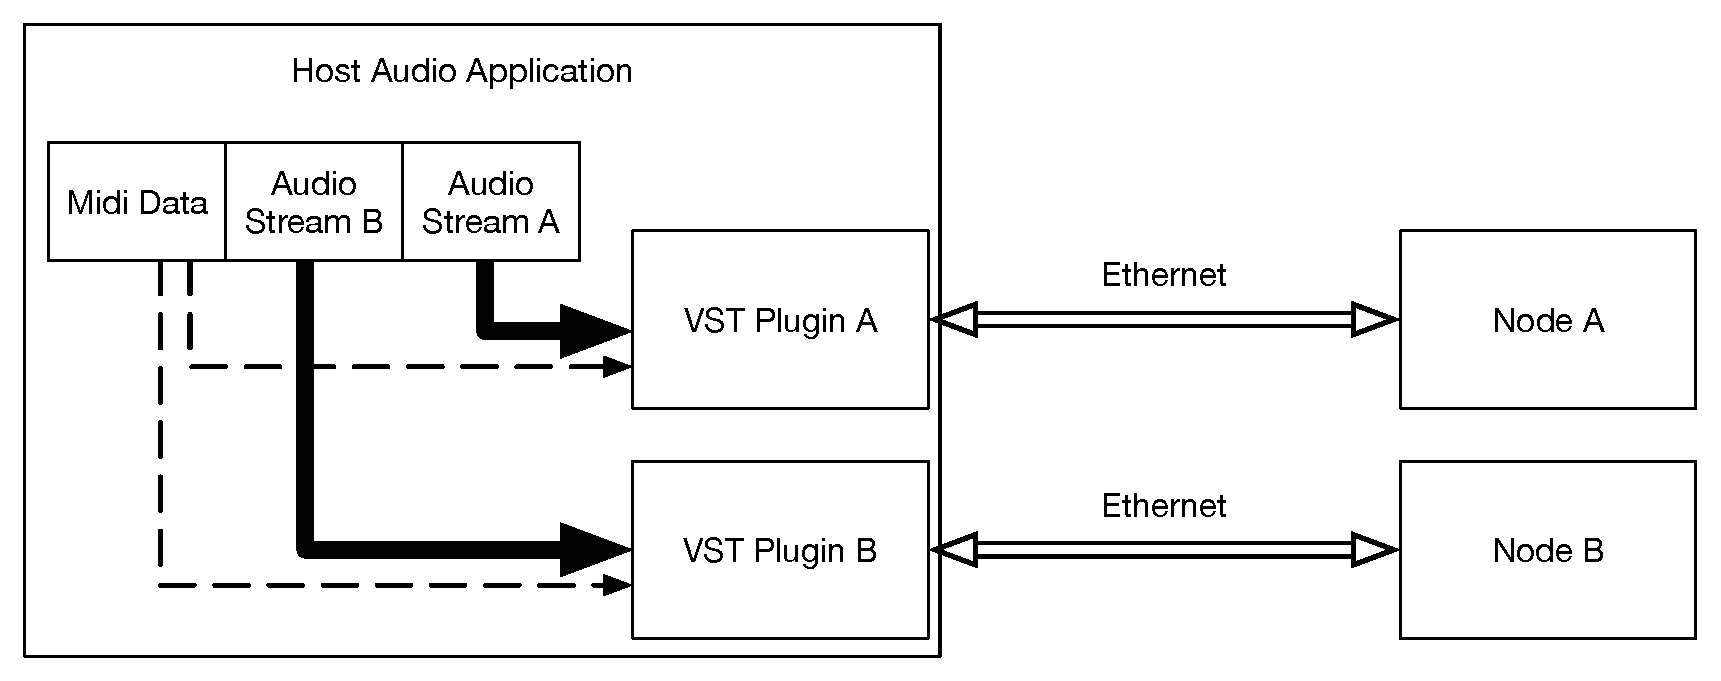
\includegraphics[width=\textwidth]{assets/distribution_1to1.pdf}
    \caption{Each Plugin Distributes to One Node}
    \label{fig:one_to_one}
\end{figure}

\begin{figure}[H]
    \centering
    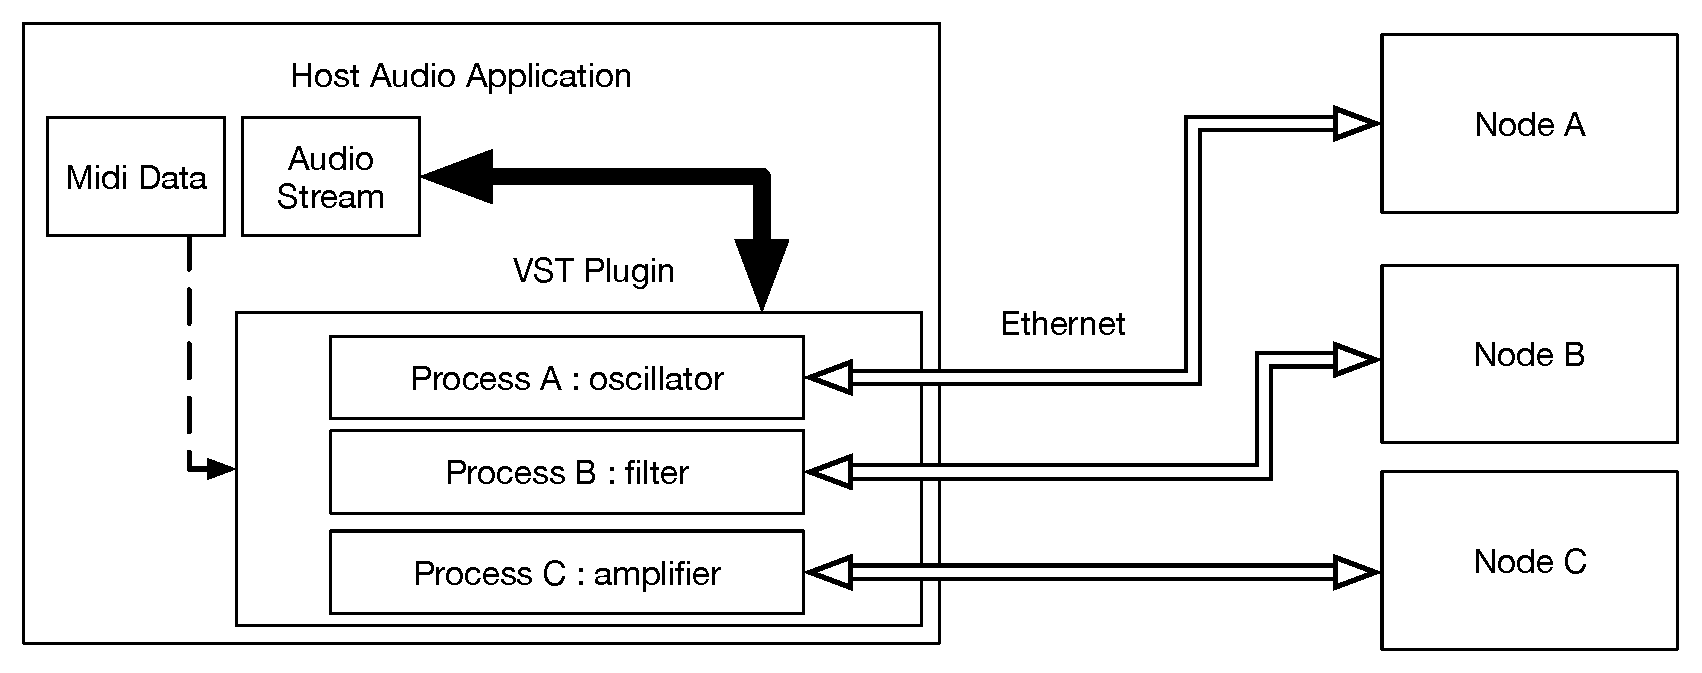
\includegraphics[width=\textwidth]{assets/distribution_perprocessor.pdf}
    \caption{Each Process Block Distributes to a Node}
    \label{fig:perproccessor}
\end{figure}

\begin{figure}[H]
    \centering
    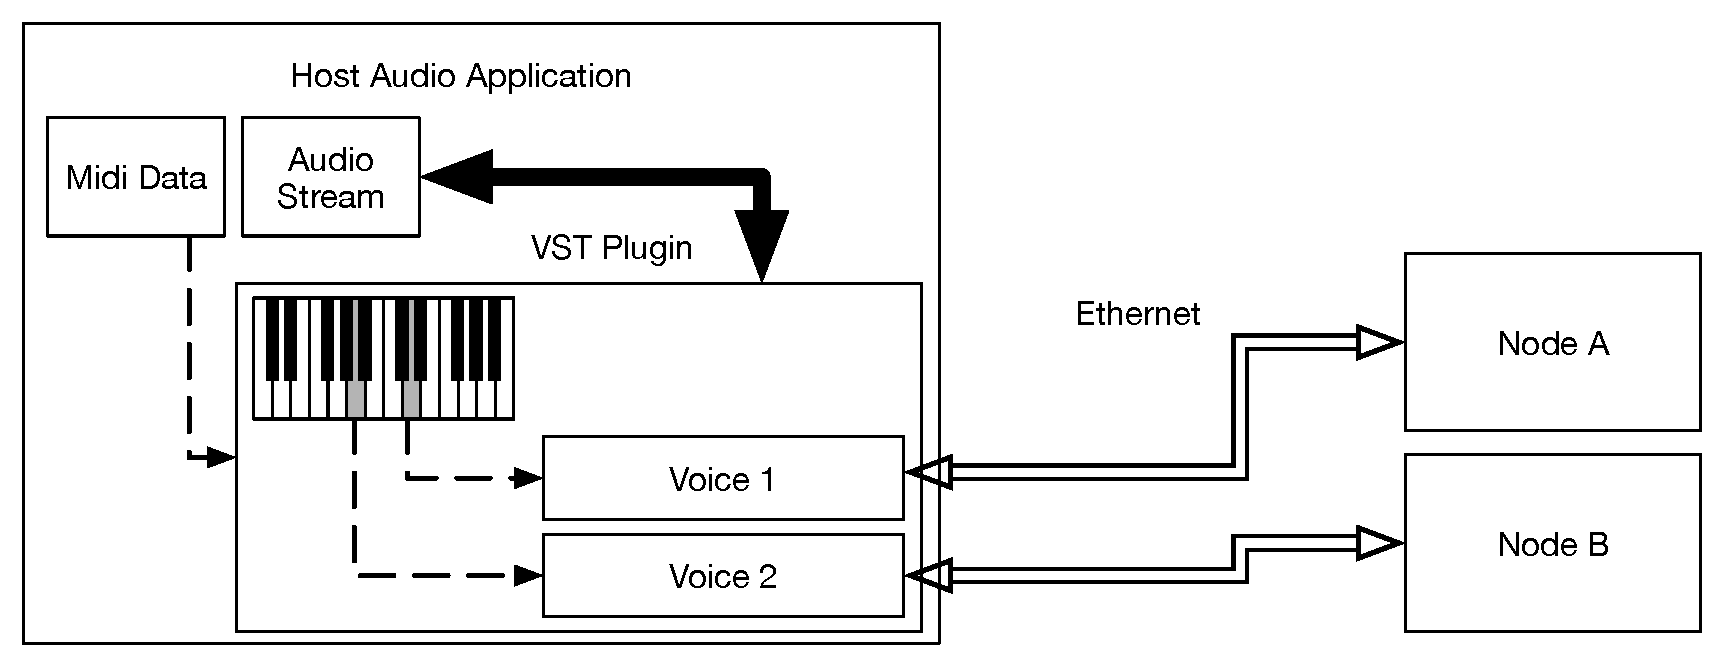
\includegraphics[width=\textwidth]{assets/distribute_byvoice.pdf}
    \caption{Each Synth Voice is Distributed to a Node}
    \label{fig:pervoice}
\end{figure}

For this project the second option will be implemented for the sake of testing, although it might not be the most efficient implementation.